% Type de document
\documentclass[a4paper,11pt,fleqn]{report}

% Chargement des extensions
\usepackage[latin1]{inputenc}
\usepackage[francais]{babel}
\usepackage{graphicx}
\usepackage{amsfonts}
\usepackage{amssymb}
\usepackage{amsmath}

\author{Guillaume SEGADO \and Oc\'eane RENNESSON}
% Début du document
\begin{document}
	
	\begin{titlepage}
	\begin{center}
\includegraphics[width=0.90\textwidth]{./logoimac.jpg}\end{center}
	\vspace*{2cm}
	\hrule
	\begin{center} {\Huge PROJET DE MATHEMATIQUES}\end{center}
	\vspace*{0.5cm}
	\begin{center} \begin{em}{\LARGE $\bigotimes\unlhd$ Trifocal Tensor $\unrhd\bigotimes$}\end{em}\end{center}
	\hrule
	\vspace*{5cm}
	 {\Large Projet r\'alis\' par Guillaume Segado \& Oc\'eane Rennesson sous la direction de M. NOZICK dans le cadre du cours de math\'ematiques d'IMAC 2e ann\'e}
	\vspace*{1cm}
	\begin{center}D\'ecembre 2012 - Janvier 2013 \end{center}
	\end{titlepage}
	

	\Huge{SOMMAIRE :}
	\vspace*{2cm}
	\\
	\Large{INTRODUCTION}
	\\\\\\
	\LARGE{I - Le Tenseur}
	\\
	\large{\begin{enumerate}
	\item{ Mod\'elisation} \\
	\item{ La Matrice A} \\
	\item{ Calcul du Tenseur} \\}
	\end{enumerate}
	\LARGE{II - Le Transfert}
	\\
	\large{\begin{enumerate}
	\item Les Cas du Transfert \\
	\item Les \'equations de transfert \\
	\item Le calcul du point \\
	\end{enumerate}}
	\LARGE{III - R\'esultats et Bilan}
	\\
	\large{\begin{enumerate}
	\item R\'esultats tests \\
	\item Checking des objectifs \\
	\item Am\'eliorations possibles \\
	\item Appr\'eciation du projet \\
	\end{enumerate}}
	\\
	\vspace*{2.5cm}
	\Huge{\bold{INTRODUCTION :}}
	\\
	\vspace*{2cm}
	\\
	\normalsize{
	\textbf{R\'esum\'e du projet :}
	\\ Ce projet traite du domaine de la vision par ordinateur et de la g\'eom\'etrie projective. Nous disposons de trois images d'une m\^eme sc\`ene mais prises avec des points de vue diff\'erents, gr\^ace \`a l'outil math\'ematique qu'est le tenseur, nous pouvons, \`a partir de la position des deux points similaires sur deux images, retrouver la position du point correspondant sur la troisi\`eme image. Pour cela, on doit dans un premier temps calculer le tenseur trifocal entre trois images, puis r\'ealiser le transfert de point en utilisant le tenseur.\\}
	
	\normalsize{
	\textbf{Applications possibles ?}\\
	\\ Nous prenons l'exemple particulier de trois images avec un tenseur trifocal, mais nous pouvons g\'en\'eraliser cette \'etude avec plusieurs images et ainsi reconstruire en 3D un objet \`a partir d'images 2D. Nous pouvons aussi prendre des sc\`enes dynamiques avec 3 cam\'eras par exemple.}
		
		\\Notre objectif est donc de coder en C++ (avec la SDL) un tenseur trifocal entre 3 images et de r\'ealiser le transfert de points. \\\\\\
		\begin{em}Pour voir le checking des objectifs demand\'es, se r\'ef\'erer au bilan.\end{em}
		
		
	\chapter{LE TENSEUR :}
	\section{\underline{Mod\'elisation :}}
	\\\\
	Un tenseur trifocal est une matrice 3 x 3 x 3. Il poss\`ede donc trois indices pour pouvoir rep\'erer un \'el\'ement stock\'e \`a l'int\'erieur. Dans tout le reste de l'\'etude, le tenseur trifocal sera not\'e $T_k^i^j$ et aura cette forme :\\\\
	\begin{center}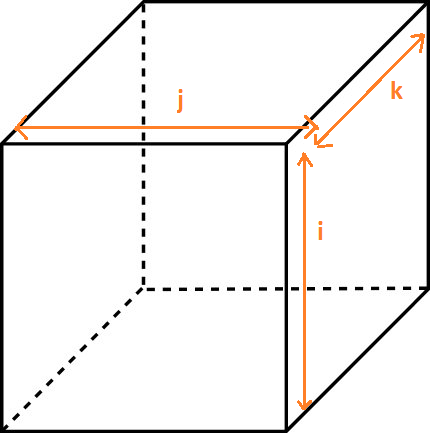
\includegraphics[width=0.60\textwidth]{./tenseur.png}\end{center}
	Nous constatons que le tenseur comprend 27 composantes et pour y acc\'eder, nous faisons varier i,j,k de 1 \`a 3 : \\ $T_1^2^2 , T_3^3^1 , T_1^1^1 , T_1^3^1 ou T_2^3^2 $ par exemple.\\\\Le premier probl\`eme qui survient est donc de mod\'eliser le tenseur. Nous avons choisi de repr\'esenter notre objet tenseur sous la forme d'un vecteur de 27 composantes pour simplifier l'approche en informatique et pour la suite avec les diff\'erentes \'equations de correspondances. Le probl\`eme est donc de passer d'un objet avec 3 'degr\'es' de libert\'e \`a un objet avec 1 'degr\'e' de libert\'e. Voici donc l'approche math\'ematique que nous avons eu :
	\\
	\begin{center}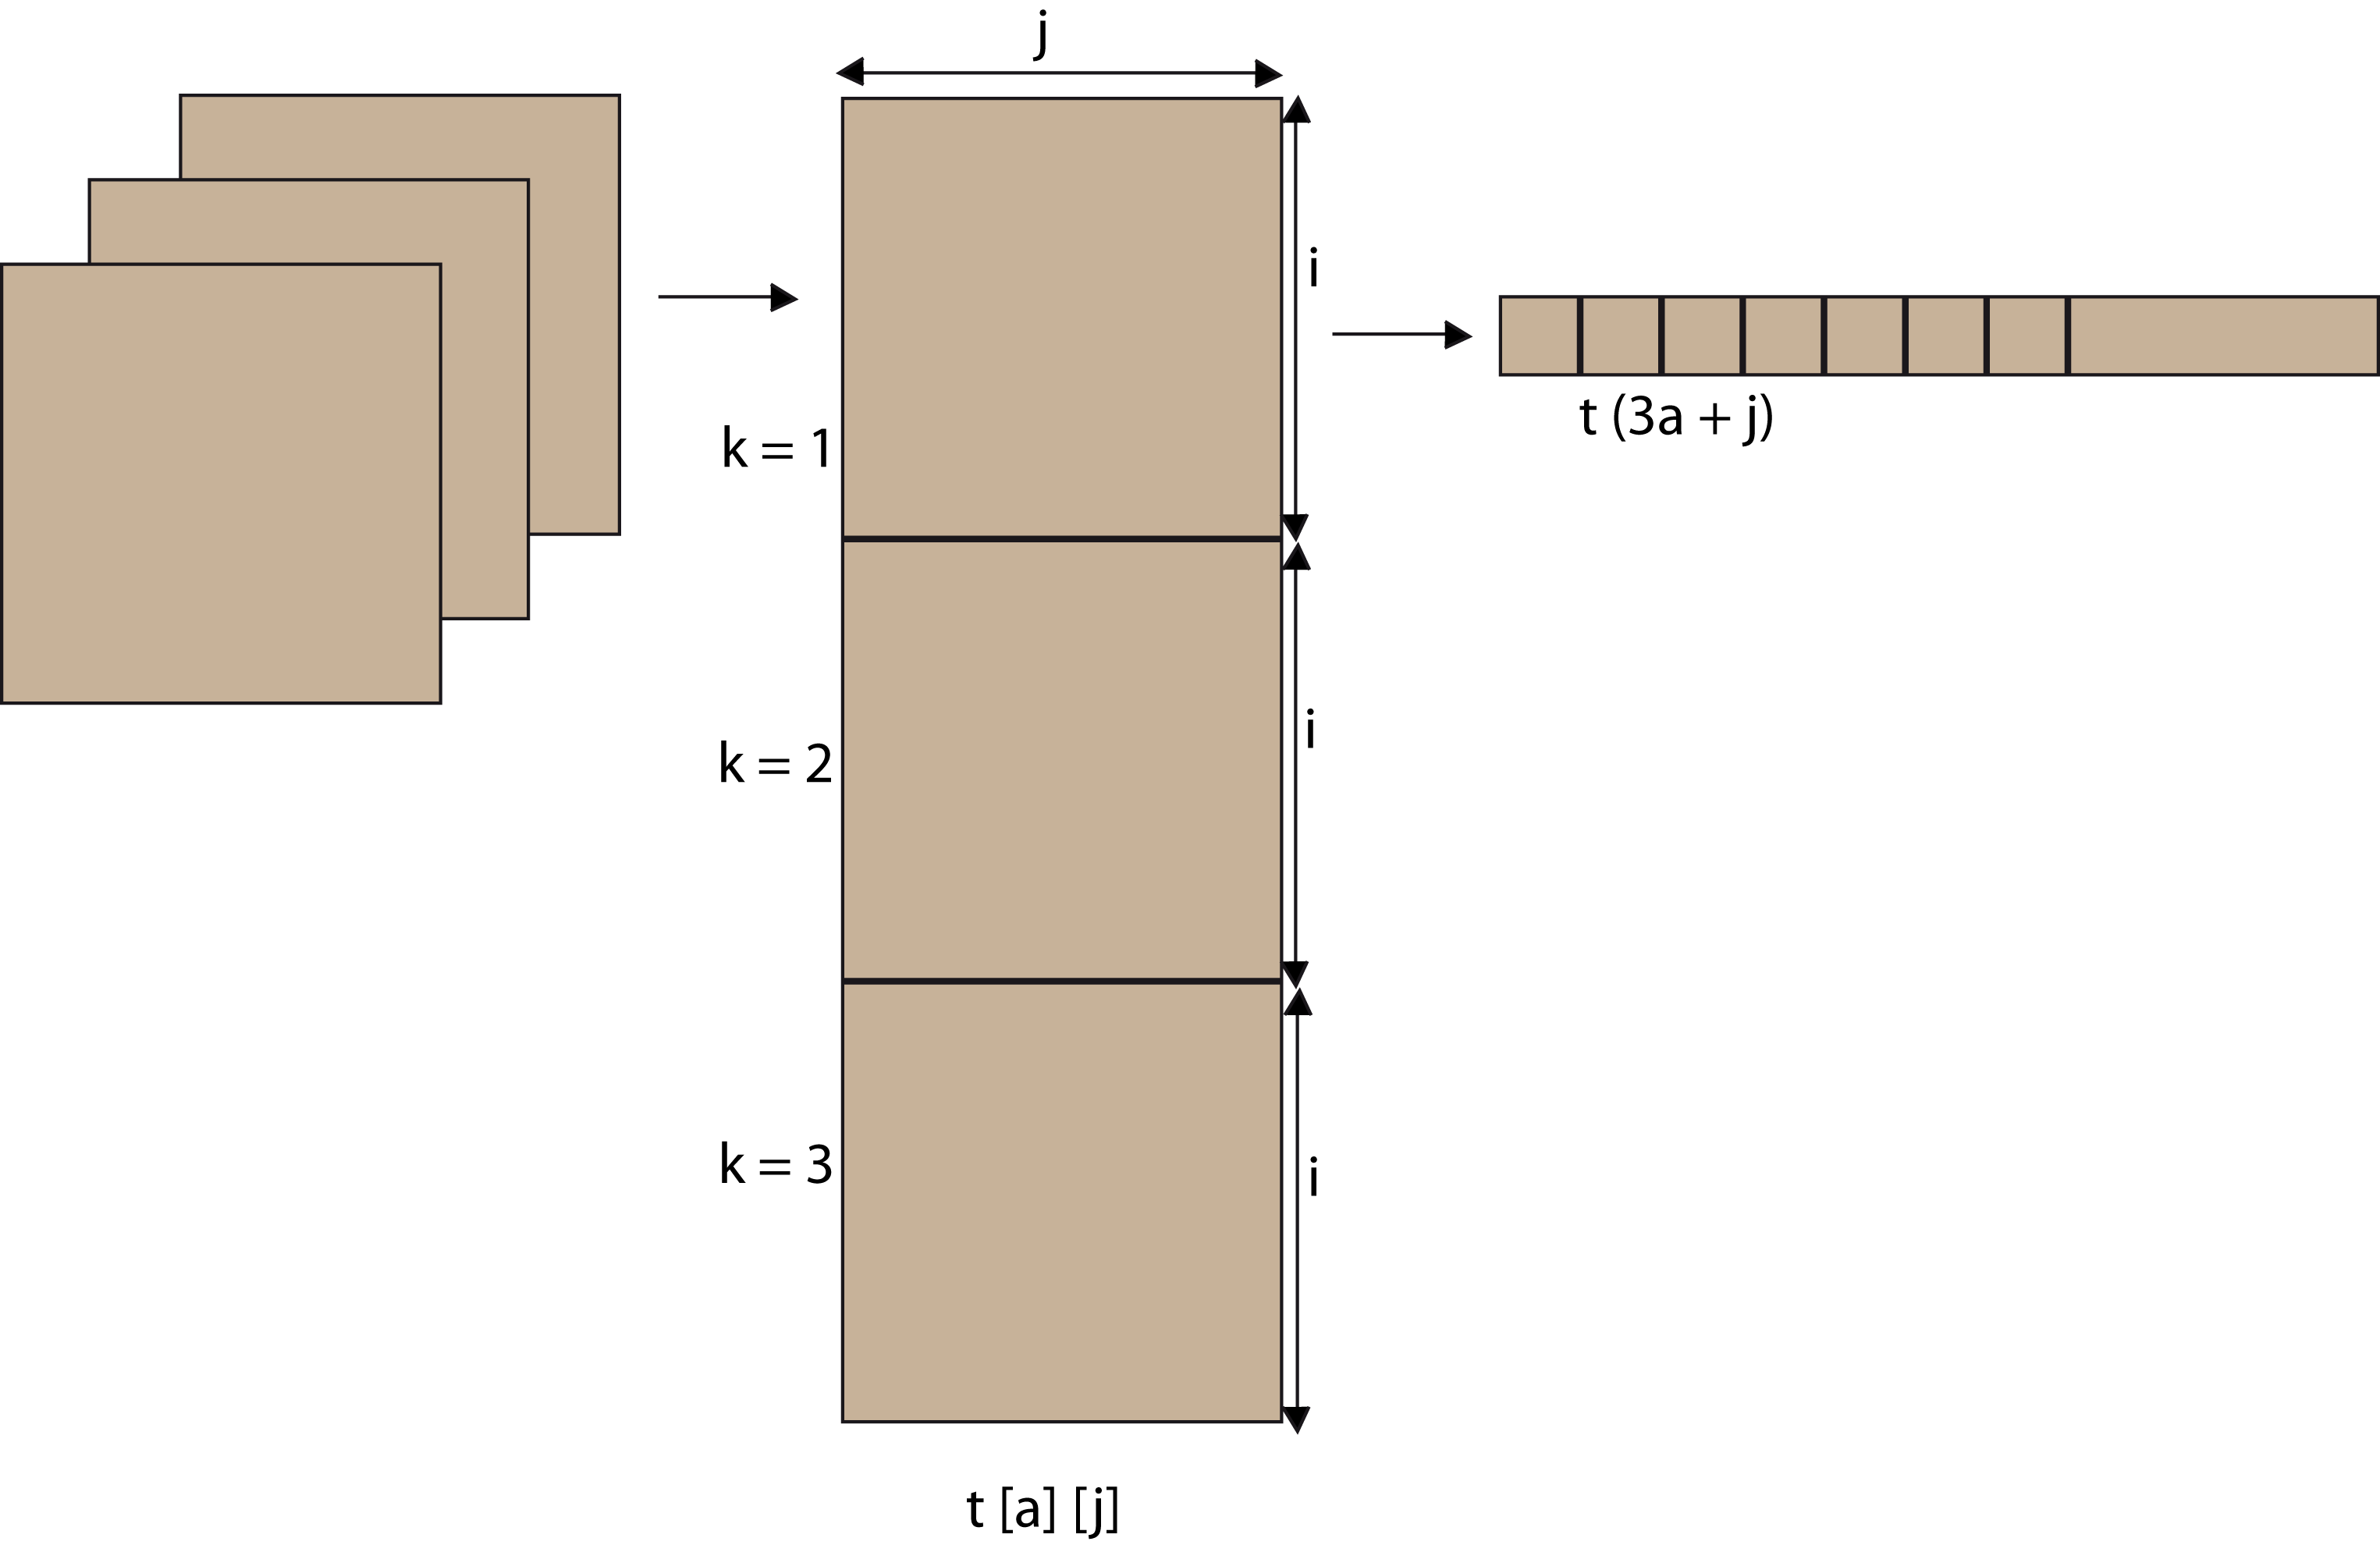
\includegraphics[width=1.2\textwidth]{./schema1.png}\end{center}
	\\\\On passe de 3 'degr\'es' de libert\'e \`a 2 'degr\'es' de libert\'e (matrice) puis 1 'degr\'e' de libert\'e (vecteur)
	'a' varie dans l'intervalle [0,8]. Il faut donc une relation pour a = f(i,k). En d\'crivant les valeurs de a, nous avons pu trouver une relation empirique qui lie a avec i et j.\\
	$a = 0 \to  i=1, k=1$\\
	$a = 1 \to  i=2, k=1$\\
	$a = 2 \to  i=3, k=1$\\
	$a = 3 \to  i=1, k=2$\\
	$a = 4 \to  i=2, k=2$\\
	$a = 5 \to  i=3, k=2$\\
	$a = 6 \to  i=1, k=3$\\
	$a = 7 \to  i=2, k=3$\\
	$a = 8 \to  i=3, k=3$\\
	Nous n'avons pas pu trouver une relation unique pour a, car il y a une sorte de dualit\'e, nous avons une relation qui fonctionne pour les 6 premiers termes ($ a = k^2 + i - 2$) de a et une relation qui fonctionne pour les 6 derniers termes ($ a = k^2 + i - 4 $) de a.
	\\
	Nous pouvons donc acc\'eder \`a un \'el\'ement du tenseur avec cet algorithme, en surchargeant l'op\'erateur () pour le tenseur :
	\\acc\'es \`a un \'el\'ement du tenseur (i,j,k)
	\\Si $k > 2$\\\\On renvoie t[$3(k^2 + i - 4) + j $]   (-1 si t[0] est d\'efini)
	\\Sinon $k < 3$\\\\On renvoie t[$3(k^2 + i - 2) + j $]   (-1 si t[0] est d\'efini)
	\\\\Comme nous allons \^etre amen\'s \`a appeller l'acc\'es au tenseur assez souvent, il faut donc que la relation soit la plus simple possible et la moins complexe, avec cette relation, nous n'appelerons qu'un seul if() \`a chaque fois.
	\\
	\\
	\\
	\section{\underline{La Matrice A :}}
	\\\\Nous avons plusieurs \'equations de correspondance qui mettent en jeu les diff\'erentes composantes du tenseur. Comme nous disposons de trois images, c'est une relation faisant intervenir trois points des trois image et le tenseur qui s'\'ecrit de cette forme l\`a : $$x^ix'^jx''^k\epsilon_j_q_s\epsilon_k_r_tT_i^q^r = 0_s_t$$
	\\Apr\`es simplification, nous utiliserons cette \'equation :
	$$\sum \limits_{k=1}^3 x_p^k(x'_p^ix''_p^3T_k^3^l - x'_p^3x''_p^3T_k^i^l - x'_p^ix''_p^lT_k^3^3 + x'_p^3x''_p^lT_k^i^3) = 0^i^l$$
	\\p repr\'esente la correspondance (il y en a n en tout), il nous faut donc au minimum 27 \'equations car le tenseur comporte 27 composantes, qui nous sont inconnues pour le moment. i et l varient de 1 \`a 2, ce qui g\'en\`ere 4 \'equations pour chaque correspondance. Il faut donc 7 correspondances de points au minimum 4x7 = 28, nous pouvons donc r\'esoudre et le syst\`eme est surd\'etermin\'e.
	\\t est notre tenseur sous la forme d'un vecteur rempli de 27 inconnues dons de taille 27, nous devons donc r\'esoudre $A\vec{t} = \vec{0}$ avec $\vec{0}$ est le vecteur nul de dimension 4n et A une matrice de taille 4n x 27
\\
\\ Notre approche pour remplir A a \'et\'e la suivante :\\
Nous avons \'ecrit sur papier dans l'ordre les 27 \'el\'ements de t, c'est \`a dire : $T_1^1^1$ $T_1^1^2$ $T_1^1^3$ $T_1^2^1$
Nous avons fait varier i, l et k et nous avons regard\'e les diff\'erentes composantes qu'il pouvait y avoir. Nous avons constat\'e que parfois pour une inconnue, il y avait n composantes, parfois 2n composantes et parfois 4n composantes.
\\ Nous avons ensuite \'etudi\'e les r\'ep\'etitions qu'il pouvait y avoir. Nous en avons trouv\'e deux grandes : \\\\pour chaque p allant de 0 \`a n
\\\\et pour k allant de 1 \`a 3.\\\\
Le sch\'ema \`a coder qui nous a paru le plus simple est de remplir par 'bloc' la grande matrice A. voici nos blocs d\'etermin\'es :
\\
\begin{center}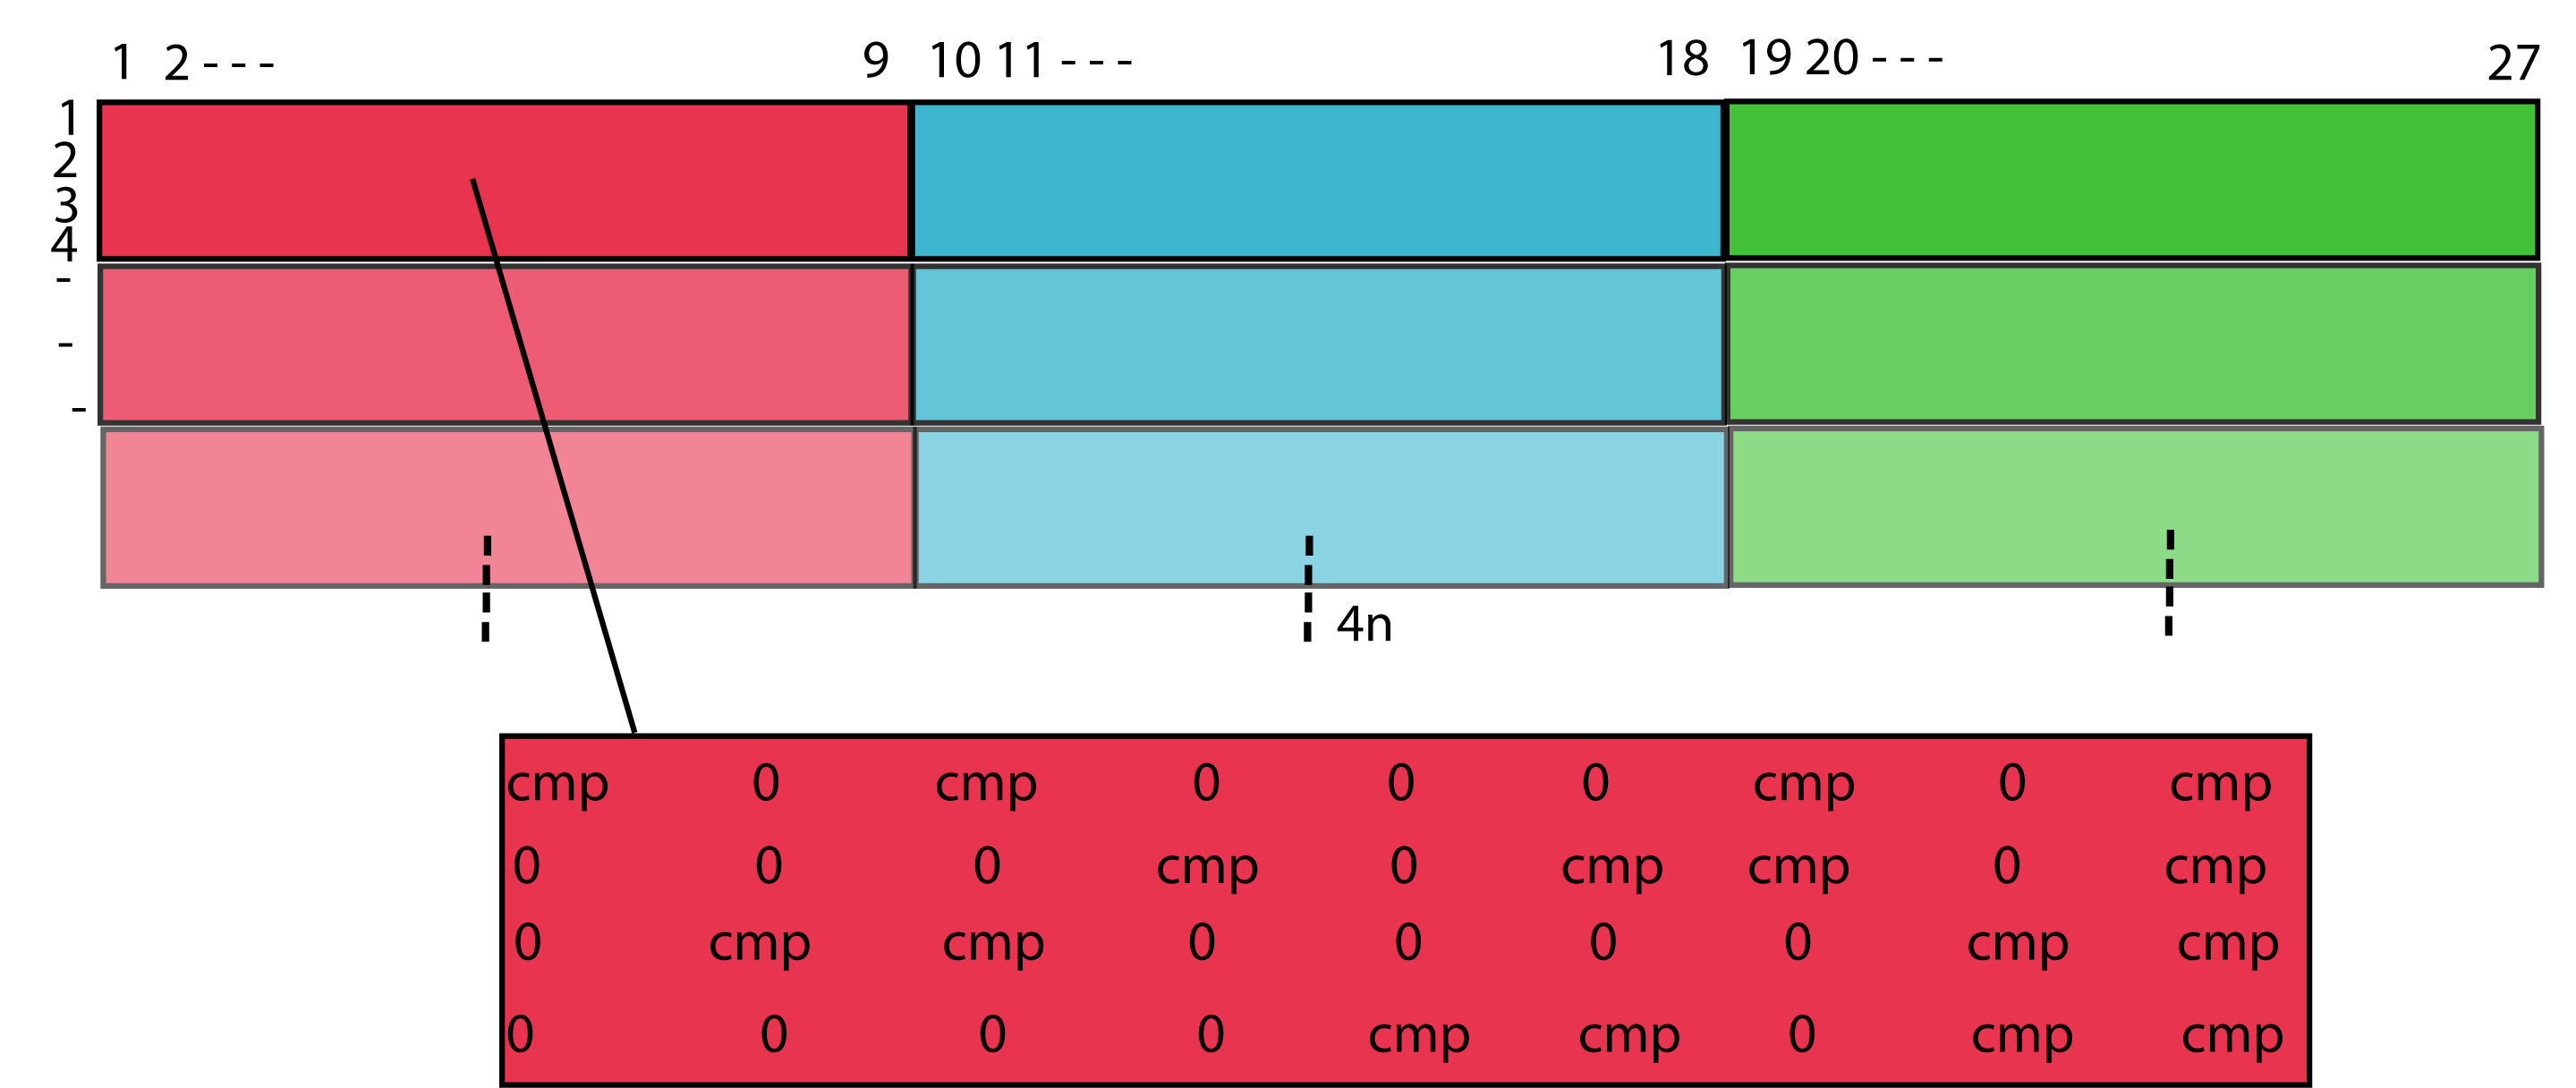
\includegraphics[width=1.2\textwidth]{./schema2.png}\end{center}
\\
'cmp' correspond \`a 'composante'.\\ Nous pouvons remplir une \`a une les colonnes $\to_{k=1} 9$ et apr\'es r\'ep\'eter le m\^eme sch\'ema $\to_{k=2} 18$ puis $\to_{k=3} 27$. Pour remplir  chaque colonne, on peut boucler 4 par 4 n fois, selon le nombre de correspondances. Donc en g\'en\'eral, on remplit par bloc de 4x9 = 36 composantes. Etant donn\'e que nous avons analys\'e un bloc, on remarque que chaque bloc est compos\'e de 20 z\'ros donc nous avons 16 composantes \`a rentrer par bloc. Nous avons choisi de faire deux boucles, une premi\`ere sur p de 1 \`a n et une deuxi\`eme \`a l'int\'erieur sur k allant de 1 \`a 3.\\\\C'est un choix de ne pas avoir fait de boucle faisant varier i et l, car i et l ne prennent que deux valeurs, 1 ou 2 et faire une boucle pour deux valeurs ce qui n'est pas assez pour faire une boucle, c'\'tait un choix de rentrer en dur les valeurs de i et l dans le bloc qui se r\'epetera selon n et selon k.
\\
\\On cr\'ee A avec le nombre de correspondance 4n en ligne et 27 en colonne. A est une matrice de Eigen. Nous initialisons A avec des zeros pour chaque composante puis nous la remplissons par bloc. Nous avons aussi au pr\'ealable stock\'e dans 3 matrices de Eigen les points $x_p$ de l'image 1, $x'_p$ de l'image 2 et $x''_p$ de l'image 3 tri\'es par correspondances (l'utilisateur charge ses points ou il les rentre manuellement en faisant les correspondances au clic). 

	\\
	\\
	\\
	\section{\underline{Le Calcul du Tenseur :}}
	\\\\Nous disposons de A maintenant, pour r\'esoudre $A\vec{t} = \vec{0}$, nous pouvons utiliser la SVD sur A. Eigen nous fournit un outil de SVD. La SVD va d\'ecomposer A  en $A = UDV^T$. Nous avons v\'erifi\'e que les \'el\'ements de D soient bien tri\'es par valeurs d\'ecroissantes. Nous trouvons la solution du syst\`eme, c'est \`a dire les 27 inconnues de t sur la derni\`ere colonne de $V^T$, $V^T$ a 27 colonnes, nous prenons donc la $27^{\`eme}$. Le choix s'est port\'e sur la SVD, car c'est une m\'ethode robuste, rapide et fiable. En effet nous obtenons des r\'esultats satisfaisants plus les correspondances sont pr\'ecises (se r\'ef\'erer \`a Bilan et R\'esultats).
	\\\\
	Nous conservons la solution dans le tenseur instanci\'e dans le main tout simplement en rentrant les valeurs de la solution dans l'ordre dans le tenseur sous forme de vecteur. Nous n'avons pas besoin de r\'earranger sous forme de tenseur car nous avons une surcharge d'op\'erateur


\chapter{LE TRANSFERT :}
\section{\underline{Les cas du transfert :}}
\\\\
	Il y a trois cas pour le transfert de point.
	\\\\Si l'utilisateur veut transf\'erer un point vers l'image 3, il a donc cliqu\'e sur deux points correspondants dans l'image 1 & 2. Nous connaissons donc x et x' (par convention) et nous nous proposons de lui trouver la position du point x'' sur l'image 3.
	\\\\Si l'utilisateur veut transf\'erer un point vers l'image 2, il a donc cliqu\'e sur deux points correspondants dans l'image 1 & 3. Nous connaissons donc x et x'' (par convention) et nous nous proposons de lui trouver la position du point x' sur l'image 2.
	\\\\Si l'utilisateur veut transf\'erer un point vers l'image 1, il a donc cliqu\'e sur deux points correspondants dans l'image 2 & 3. Nous connaissons donc x' et x'' (par convention) et nous nous proposons de lui trouver la position du point x sur l'image 1.
	\\\\
	Pour faciliter la visualisation, quand l'utilisateur choisit ses deux points pour le transfert, au moment o\`u il clique sur un pixel, un disque en couleur appara\^it (son centre est le pixel choisi). Puis nous lui montrons son r\'esultat du transfert sur la troisi\`eme image par un cercle non plein. Nous choississons de ne pas effacer ces cercles, ainsi, l'utilisateur peut tester plusieurs combinaisons, et r\'ealiser les trois types de transfert comme il le souhaite, dans l'ordre voulu.
\\\\
\section{\underline{Les \'equations de transfert :}}
\\\\\\
	Comment transf\'erer un point sur une autre image ?\\\\
	Cette fois ci, on dispose du tenseur trifocal rempli ainsi que de deux points correspondants sur deux images.
	Nous cherchons les coordonn\'ees du troisi\`eme point, c'est \`a dire par exemple : $(x''^1,x''^2)$ ou $(x'^1,x'^2)$ ou $(x^1,x^2)$. Mais dans \mathbb{P} l'espace projectif, nous ne devons pas n\'egliger la coordonn\'ee homog\`ene. En effet, elle va nous \^etre tr\`es utile lorque nous devrons repasser en coordonn\'ees cart\'esiennes.
	\\
	\\
	Nous utilisons donc les m\^emes \'equations que celle du calcul du tenseur, mais nous n'avons plus que 3 inconnues : Les 3 coordonn\'ees du point \`a transf\'erer.
	$$\sum \limits_{k=1}^3 x^k(x'^ix''^3T_k^3^l - x'^3x''^3T_k^i^l - x'^ix''^lT_k^3^3 + x'^3x''^lT_k^i^3) = 0^i^l$$
	\\
	Nous avons donc proc\'ed\'e avec la m\^eme d\'emarche, nous avons fait varier i et l de 1 \`a 2 et \'etudi\'e les diff\`erentes composantes pour chacune des trois coordonn\'ees. Nous avons fait varier i et l dans cette ordre l\`a.
	\\$i=1$ $k=1$
	\\$i=2$ $k=1$
	\\$i=1$ $k=2$
	\\$i=2$ $k=2$\\\\Cel\`a nous a donc g\'en\'er\'e 4 \'equations pour 3 inconnues, nous pouvons donc r\'esoudre avec les m\^emes outils, entre autre, la SVD. Nous allons donc cr\'eer avec une matrice G de taille 4x3 et r\'esoudre le syst\`eme $G\vec{x''} = \vec{0}$ par exemple.\\Nous obtenons ces trois syst\`emes pour les trois cas diff\'erents (cmp pour composante):\\\\
	Le transfert pour x'' (vers la troisi\`eme image)\\
	$$ \begin{pmatrix}
	cmp&0&cmp \\
	cmp&0&cmp \\
	0&cmp&cmp \\
	0&cmp&cmp \\
	\end{pmatrix}\begin{pmatrix}x''^1\\x''^2\\x''^3\end{pmatrix} = \begin{pmatrix}0\\0\\0\\0\end{pmatrix} $$
	\\\\Le transfert pour x' (vers la deuxi\`eme image)\\
	$$ \begin{pmatrix}
	cmp&0&cmp \\
	0&cmp&cmp \\
	cmp&0&cmp \\
	0&cmp&cmp \\
	\end{pmatrix}\begin{pmatrix}x'^1\\x'^2\\x'^3\end{pmatrix} = \begin{pmatrix}0\\0\\0\\0\end{pmatrix} $$
	\\\\Le transfert pour x (vers la premi\`ere image)\\\\
	$$ \begin{pmatrix}
	cmp&cmp&cmp \\
	cmp&cmp&cmp \\
	cmp&cmp&cmp \\
	cmp&cmp&cmp \\
	\end{pmatrix}\begin{pmatrix}x^1\\x^2\\x^3\end{pmatrix} = \begin{pmatrix}0\\0\\0\\0\end{pmatrix} $$
	\\\\Apr\`es avoir d\'evelopp\'e les \'equations de transfert, nous avons remarqu\'e que pour chaque cas, 
	dans les composantes des matrices G, \'etaient pr\'esents tous les \'el\'ement du tenseur, il n'en manquait pas un.\\Pour remplir les matrices G, nous faisons une boucle sur k qui varie de 1 \`a 3, car les composantes sont des sommes sur k, donc des morceaux se r\'epetent. Encore une fois, par choix, nous ne faisons pas de boucle sur i et j qui varient seulement de 1 \`a 2.\\\\
	Pour g\'erer les trois cas, la fonction 'transfert' est adapt\'ee pour remplir la matrice G correctement.
	
	\\\\
\section{\underline{Le Calcul du point :}}
	\\\\Pour calculer le point transf\'er\'e, il nous faut r\'esoudre le syst\`eme : $G\vec{x''} = \vec{0}$. Nous allons utiliser les m\^emes outils de la matrice A pour trouver la solution. On pratique la SVD sur G. et nous r\'ecup\'erons la solution sur la derni\`ere colonne : la $3^{\`eme}$.\\
	Nous obtenons un vecteur solution avec des valeurs tr\`es petites. En effet, la SVD calcule le vecteur solution $\vec{x}$ tel que $||\vec{x}|| = 1$. De plus pour pouvoir repasser dans l'espace euclidien et ainsi avoir des r\'esultats coh\'erents, il faut diviser les coordonn\'ees solutions par la coordonn\'ees homog\`ene. En effet, on obtient des r\'esultat concluant, le transfert est effectu\'e. Par exemple, nous obtenons : \\\\
	$\begin{pmatrix}0,8786\\0,4776\\0,005351\end{pmatrix} \doteq \begin{pmatrix}164,19\\89,25\\1\end{pmatrix}$
	
	\chapter{RESULTATS ET BILAN :}
	\section{\underline{Les R\'esultats :}}
	\\\\
	\textbf{Test avec les images du sujet}\\
	Le programme se lance (-h pour activer l'aide). Les images sont charg\'ees. L'utilisateur lance alors le chargement de listes pr\'e-construites, il appuie alors sur la touche 'c' pour le mode de chargement de listes.
	\begin{center}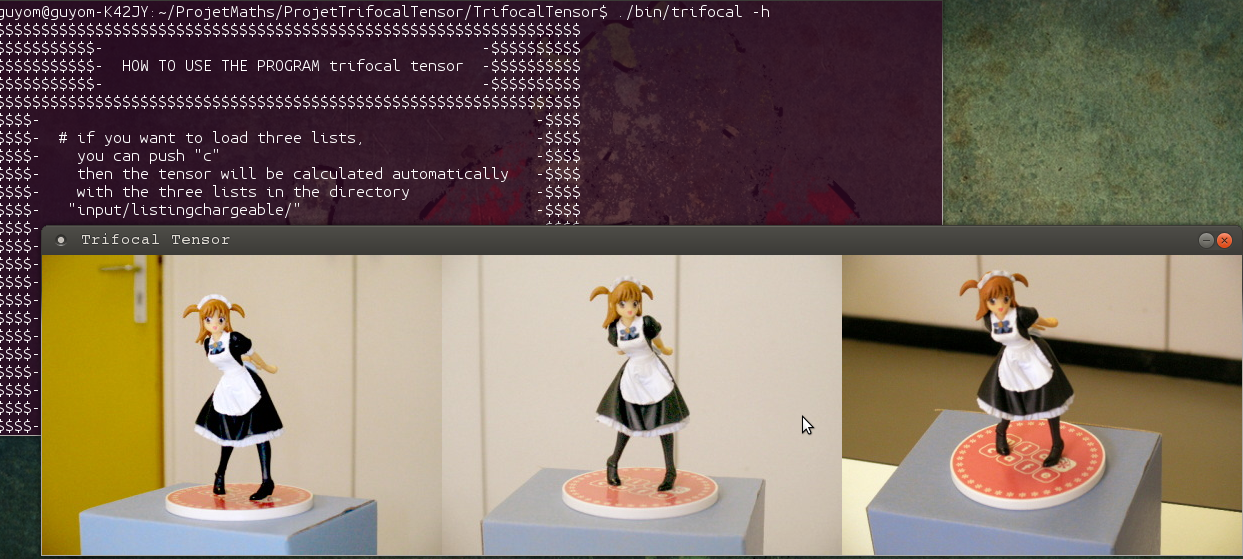
\includegraphics[scale=0.50]{./capture1.png}\end{center}\\
	Les points sont charg\'es, et des disques de couleur apparaissent sur les images pour montrer \'a l'utilisateur les points qu'il vient de charger pour le calcul du tenseur. Le programme attend 2 secondes pour passer ensuite au mode de transfert apr\'es avoir calcul\'e le tenseur et effac\'e des images les points de d\'eparts.
	\begin{center}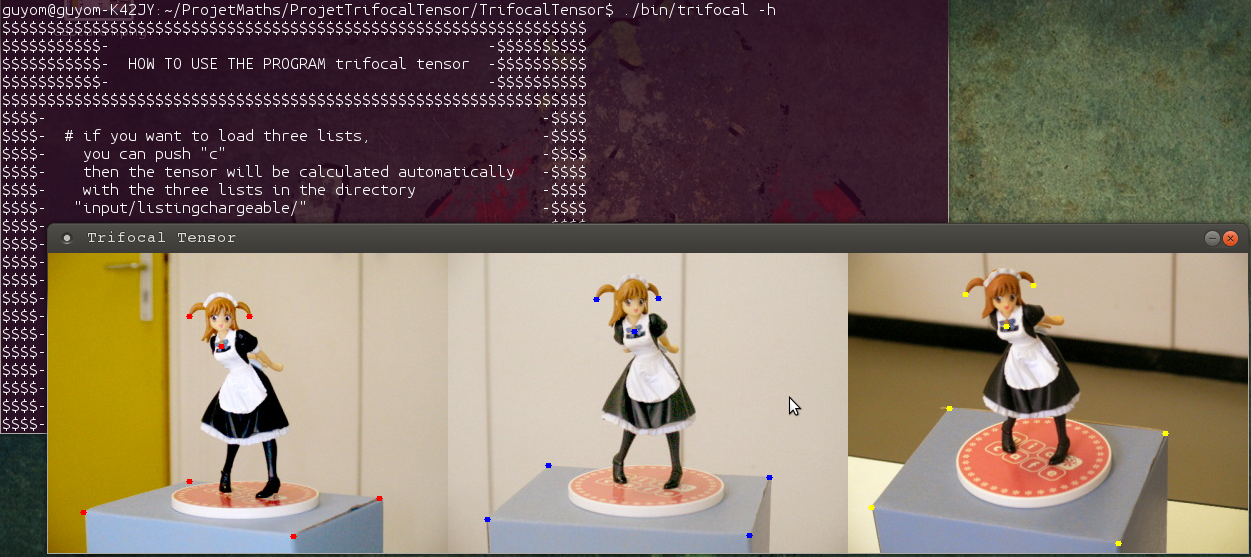
\includegraphics[scale=0.50]{./capture2.png}\end{center}\\
	L'utilisateur passe en mode transfert, il clique sur deux points correspondants sur deux images.
	\begin{center}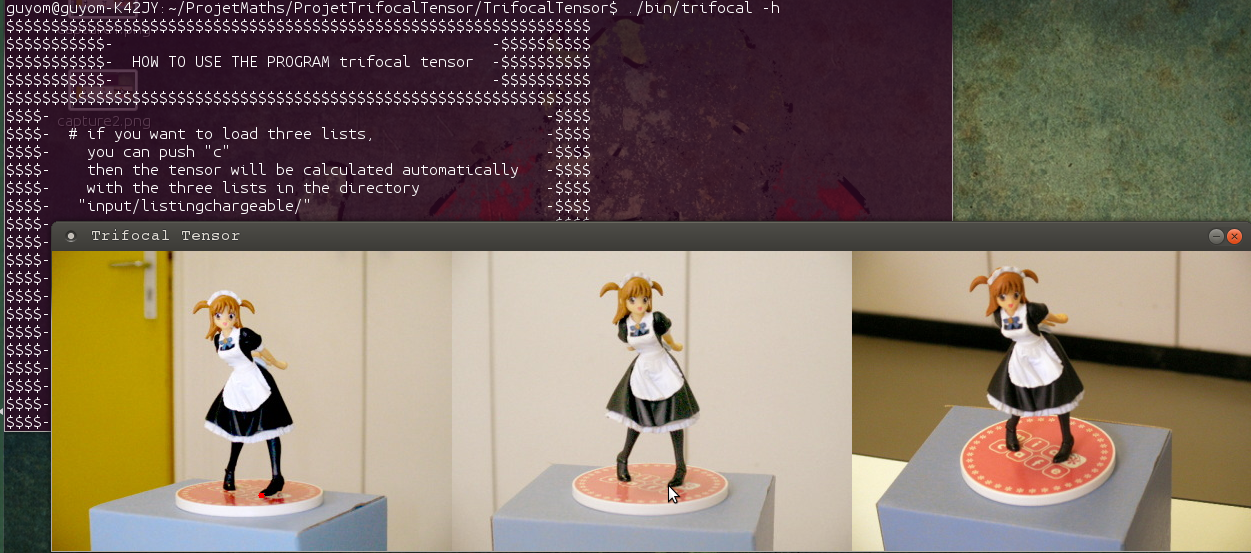
\includegraphics[scale=0.50]{./capture3.png}\end{center}\\
	Puis un cercle de couleur non rempli se dessine sur la troisi\`eme image afin de montrer la position du point transf\'er\'e. A chaque nouveau test, les cercles ne sont pas effac\'es pour laisser \`a l'utilisateur le choix d'appr\'ecier ses r\'esultats.
	\begin{center}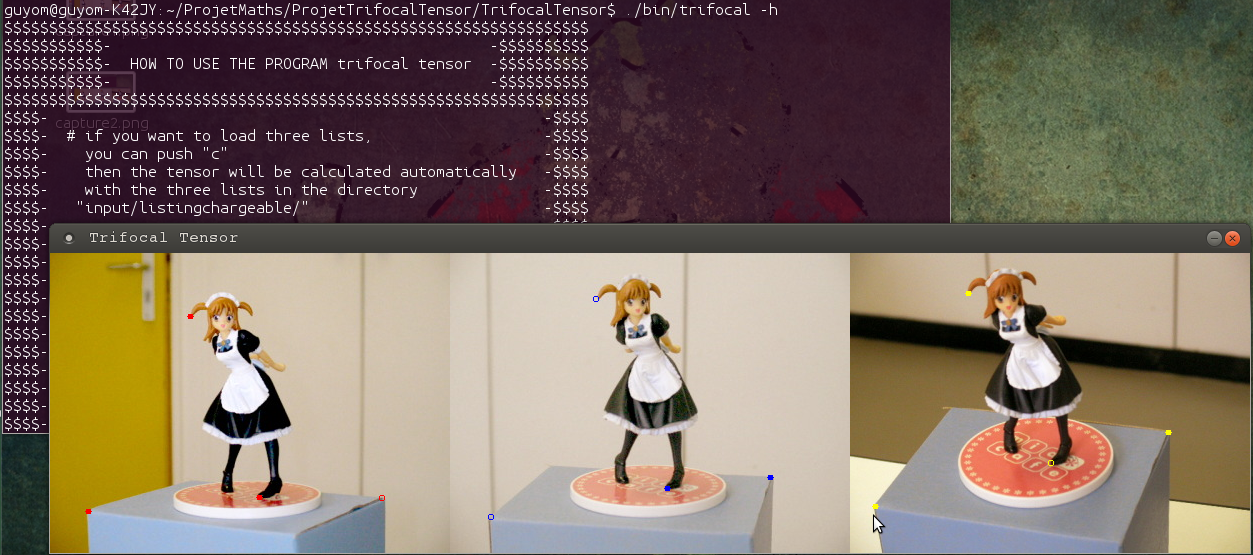
\includegraphics[scale=0.50]{./capture4.png}\end{center}\\\\
	\textbf{Test avec nos images}\\
	Et oui, Cartman s'est port\'e volontaire pour participer au projet trifocal tensor, il \`a m\^eme pos\' pour nous.L\`a pareil, l'utilisateur va rentrer des points, mais cette fois, il ne va pas charger des listes pr\'e-construites, il va passer en mode manuel et cliquer sur ses correspondances dans l'ordre (au minimum 7). Une fois fini, l'utilisateur doit appuyer sur la touche 'f' pour calculer le tenseur et passer au mode de transfert de points. Les correspondances sont sauvegard\'ees sous forme de fichier.list mis en page de cette facon l\`a :\\\\
row 11\\
col 3\\
 \\\\
104 119   1\\
262 189   1\\
173 144   1\\
161 230   1\\
 99 171   1\\
223 141   1\\
269 212   1\\
163 229   1\\
 81 213   1\\
388  83   1\\
 69  90   1\\
	\begin{center}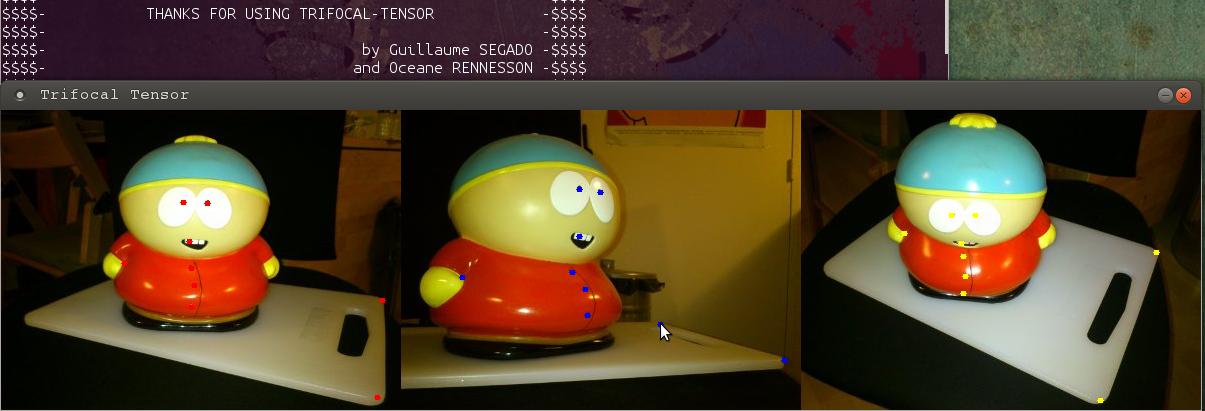
\includegraphics[scale=0.50]{./cartman1.png}\end{center}\\
	Il passe ensuite au mode transfert qui fonctionne sur le m\^eme principe que ci-dessus.
	\begin{center}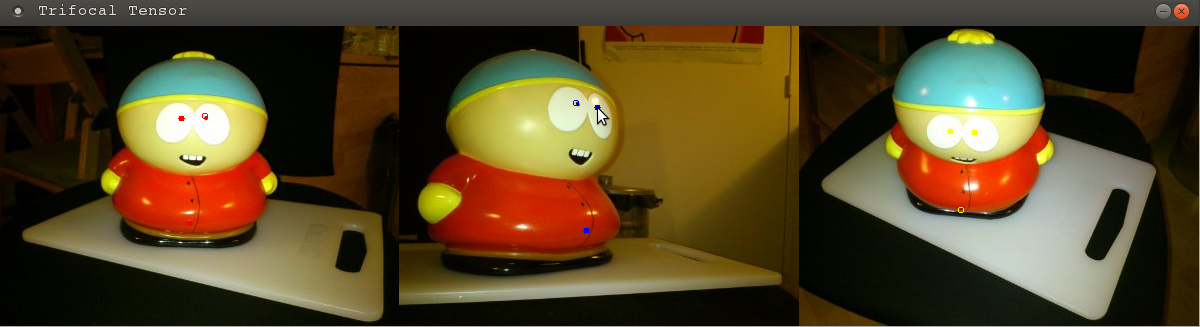
\includegraphics[scale=0.50]{./cartman2.png}\end{center}Merci Cartman\\\\
	\section{\underline{Bilan :}}
	\\\\
	\textbf{Checking des points demand\'es :}\\\\
	$\surd$ impl\'ementer un programme de gestion de tenseur trifocal.\\
	$\surd$ \^etre \'ecrit en C++\\
	$\surd$ utiliser un Makefile\\
	$\surd$ ne plus afficher de warning lors de la compilation (utilisation du flag -Werror)\\
	$\surd$ fonctionne sous Linux\\
	$\surd$ Lancement sous console avec une aide en anglais qui s'affiche si l'option -h est ajout\'e \`a la commande d'ex\'ecution\\
	$\surd$ n'utilise que l'interface de la SDL\\
	$\surd$ chargement de listes d\'ej\`a \'etablies et correspondances cliquables ainsi que sauvegarde dans un fichier. la sauvegarde s'effectue sous la bonne forme, mais pour le chargement de liste, ce n'est pas la bonne forme.\\
	$\surd$ Calcul d'un Tenseur & transfert de points (les 3 cas de transfert)\\
	$\surd$ Affichage de cercles ou disques pour les points selectionn\'es, charg\'es ou transf\'er\'es\\
		
	\\\\
	\textbf{Am\'eliorations possibles :}\\\\
	Il y a beaucoup d'am\'eliorations possibles pour ce programme. Par exemple au niveau de la gestion, au niveau de l'interface. On peut par exemple se tromper en effectuant un clic de point, on pourrait imaginer un 'undo' de la derni\`ere action entreprise par l'utlisateur.
	On peut aussi par exemple lors du transfert, sauvegarder les r\'esultats pour pouvoir les exploiter ou les r\'eutiliser plus tard.
	\\
	\\
	\textbf{Appr\'eciation du projet :}\\\\
	•Pour ma part, ce projet m'a beaucoup apport\'e, tant en comp\'etences informatiques qu'en comp\'etences math\'ematiques. Le probl\`eme au d\'ebut me paraissait concret, je visualisais l'utilit\'e. Mais la partie math\'ematique m'a rebut\'e car complexe \`a premi\`ere vue. Une fois que l'on pose bien le probl\`eme plusieurs fois, on trouve des r\'esultats, et on trouve du plaisir \`a voir de la coh\'erence par la suite selon les choix math\'ematiques et informatiques que l'on prend. Au niveau de l'informatique, j'ai pu me familiariser avec Eigen, et surtout d\'ecouvrir la puissance de certains outils informatiques, notamment la SVD. Et pour finir , j'ai de plus d\'evelopp\'e mes comp\'etences en \LaTeX.\\
	•Ce projet m'aura permis de d\'couvrir une nouvelle approche math\'matique permettant de r\'soudre un probl\`eme concret sur la suite d'images, et d'appr\'hender la communication en tant que groupe.
	
	
% Fin du document
\end{document}


